% TODO move section...

\section{\RU{Некоторые паттерны в бинарных файлах}\EN{Some binary file patterns}}

\EN{
All examples here were prepared on the Windows with active code page 437
\footnote{\url{https://en.wikipedia.org/wiki/Code_page_437}} in console.
Binary files internally may look visually different if another code page is set.
}
\RU{
Все примеры здесь были подготовлены в Windows с активной кодовой страницей 437
\footnote{\url{https://ru.wikipedia.org/wiki/CP437}} в консоли.
Двоичные файлы внутри могут визуально выглядеть иначе если установлена другая кодовая страница.
}

\clearpage
\subsection{\EN{Arrays}\RU{Массивы}}

\EN{Sometimes, we can clearly spot an array of 16/32/64-bit values visually, in hex editor.}
\RU{Иногда мы можем легко заметить массив 16/32/64-битных значений визуально, в шестнадцатеричном 
редакторе.}

\RU{Вот пример массива 16-битных значений.
Мы видим что каждый первый байт в паре всегда равен 7 или 8, а второй выглядит случайным:}
\EN{Here is an example of array of 16-bit values.
We see that the first byte in pair is 7 or 8, and the second looks random:}

\begin{figure}[H]
\centering
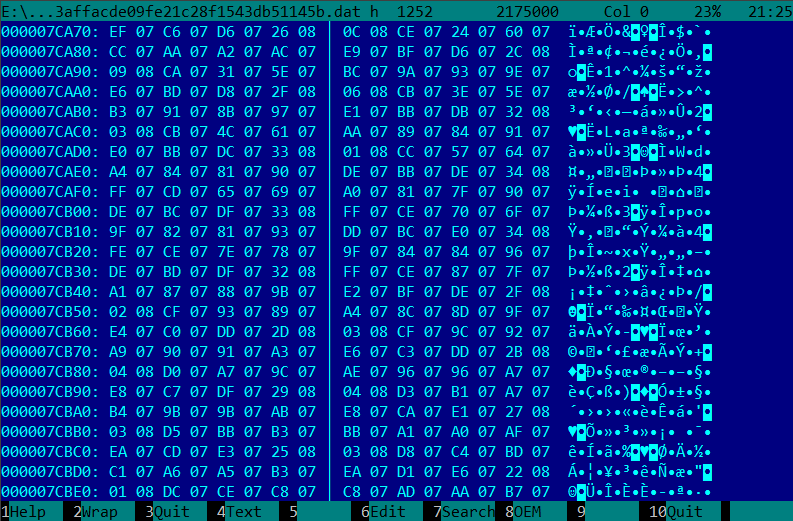
\includegraphics[scale=\NormalScale]{digging_into_code/binary/16bit_array.png}
\caption{FAR: \RU{массив 16-битных значений}\EN{array of 16-bit values}}
\end{figure}

\RU{Для примера я использовал файл содержащий 12-канальный сигнал оцифрованный при помощи 16-битного \ac{ADC}.}
\EN{I used a file containing 12-channel signal digitized using 16-bit \ac{ADC}.}

\clearpage
\index{MIPS}
\par
\EN{And here is an example of very typical MIPS code.}
\RU{А вот пример очень типичного MIPS-кода.}
\EN{As we may remember, every MIPS (and also ARM in ARM mode or ARM64) instruction has size of 32 bits (or 4 bytes), 
so such code is array of 32-bit values.}
\RU{Как мы наверное помним, каждая инструкция в MIPS (а также в ARM в режиме ARM, или ARM64) имеет 
длину 32 бита (или 4 байта),
так что такой код это массив 32-битных значений.}
\EN{By looking at this screenshot, we may see some kind of pattern.}
\RU{Глядя на этот скриншот, можно увидеть некий узор.}
\EN{Vertical red lines are added for clarity}\RU{Вертикальные красные линии добавлены для ясности}:

\begin{figure}[H]
\centering
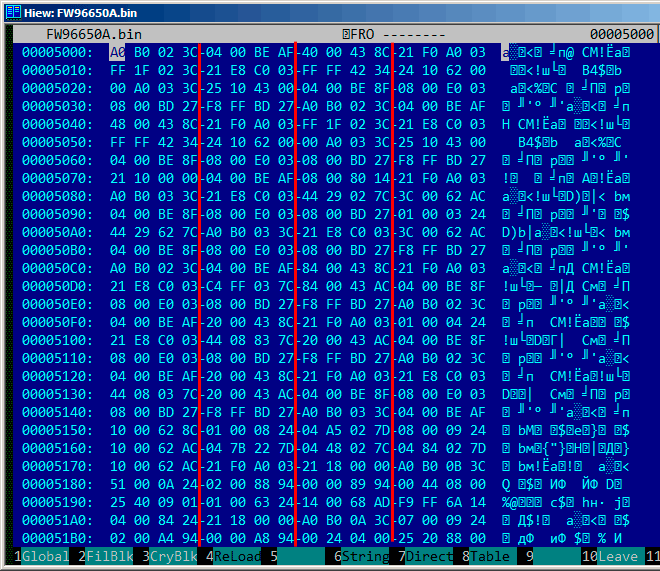
\includegraphics[scale=\NormalScale]{digging_into_code/binary/typical_MIPS_code.png}
\caption{Hiew: \EN{very typical MIPS code}\RU{очень типичный код для MIPS}}
\end{figure}

\RU{Еще пример таких файлов в этой книге}\EN{Another example of such pattern here is book}: 
\myref{Oracle_SYM_files_example}.

\clearpage
\subsection{\EN{Sparse files}\RU{Разреженные файлы}}

\ifdefined\ENGLISH
This is sparse file with data scattered anibg almost empty file.
Each space character here is in fact zero byte (which is looks like space).
This is a file to program FPGA (Altera Stratix GX device).
Of course, files like these can be compressed easily, but formats like this one are very popular in scientific and engineering software where efficient access is important while compactness is not.
\fi % ENGLISH

\ifdefined\RUSSIAN
Это разреженный файл, в котором данные разбросаны посреди почти пустого файла.
Каждый символ пробела здесь на самом деле нулевой байт (который выглядит как пробел).
Это файл для программирования FPGA (чип Altera Stratix GX).
Конечно, такие файлы легко сжимаются, но подобные форматы очень популярны в научном и инженерном ПО, где быстрый доступ важен, а компактность --- не очень.
\fi % RUSSIAN

\begin{figure}[H]
\centering
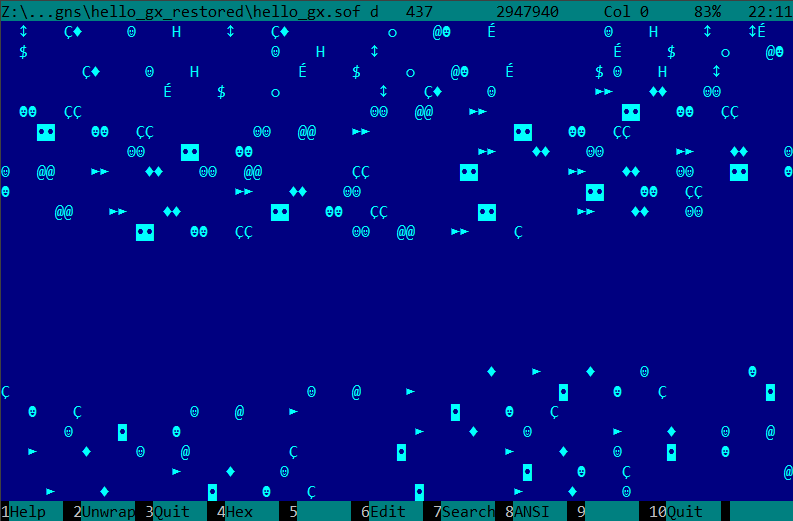
\includegraphics[scale=\NormalScale]{digging_into_code/binary/sparse_FPGA.png}
\caption{FAR: \EN{Sparse file}\RU{Разреженный файл}}
\end{figure}

\clearpage
\subsection{\EN{Compressed file}\RU{Сжатый файл}}

% FIXME \ref{} ->
\ifdefined\ENGLISH
This file is just some compressed archive.
It has relatively high entropy and visually looks just chaotic.
This is how compressed and/or encrypted files looks like.
\fi % ENGLISH

\ifdefined\RUSSIAN
Этот файл это просто некий сжатый архив.
Он имеет довольно высокую энтропию и визуально выглядит просто хаотичным.
Так выглядят сжатые и/или зашифрованные файлы.
\fi % RUSSIAN

\begin{figure}[H]
\centering
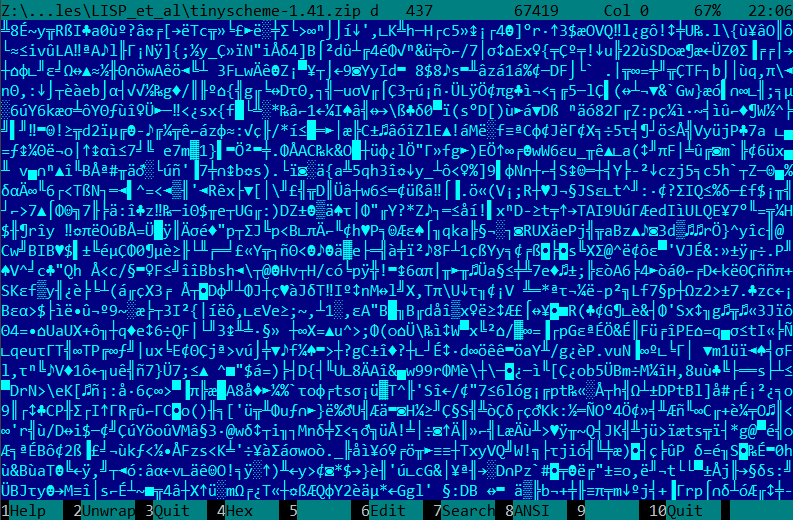
\includegraphics[scale=\NormalScale]{digging_into_code/binary/compressed.png}
\caption{FAR: \EN{Compressed file}\RU{Сжатый файл}}
\end{figure}

\clearpage
\subsection{\ac{CDFS}}

\ifdefined\ENGLISH
\ac{OS} installations are usually distributed as ISO files which are copies of CD/DVD discs.
Filesystem used is named \ac{CDFS}, here is you see file names mixed with some additional data.
This can be file sizes, pointers to another directories, file attributes, etc.
This is how typical filesystems may look internally.
\fi % ENGLISH

\ifdefined\RUSSIAN
Инсталляции \ac{OS} обычно распространяются в ISO-файлах, которые суть копии CD/DVD-дисков.
Используемая файловая система называется \ac{CDFS}, здесь видны имена файлов и какие-то довольнительные данные.
Это могут быть длины файлов, указатели на другие директории, аттрибуты файлов, итд.
Так может выглядеть типичная файловая система внутри.
\fi % RUSSIAN

\begin{figure}[H]
\centering
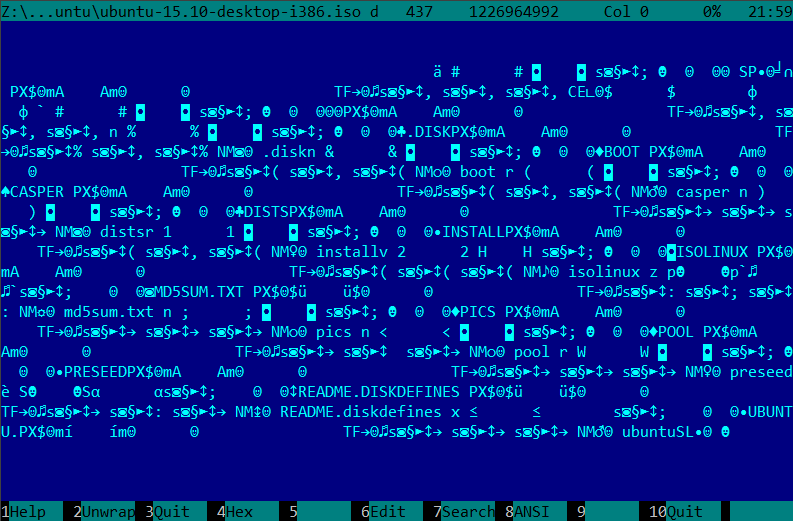
\includegraphics[scale=\NormalScale]{digging_into_code/binary/cdfs.png}
\caption{FAR: \EN{ISO file: Ubuntu 15 installation \ac{CD}}\RU{ISO-файл: инсталляционный \ac{CD} Ubuntu 15}}
\end{figure}

\clearpage
\subsection{\EN{32-bit x86 executable code}\RU{32-битный x86 исполняемый код}}

\EN{This is how 32-bit x86 executable code looks like.
It has not very high entropy, because some bytes occurred more often than others.}
\RU{Так выглядит 32-битный x86 испольняемый код.
У него не очень высокая энтропия, потому что некоторые байты встречаются чаще других.}

\begin{figure}[H]
\centering
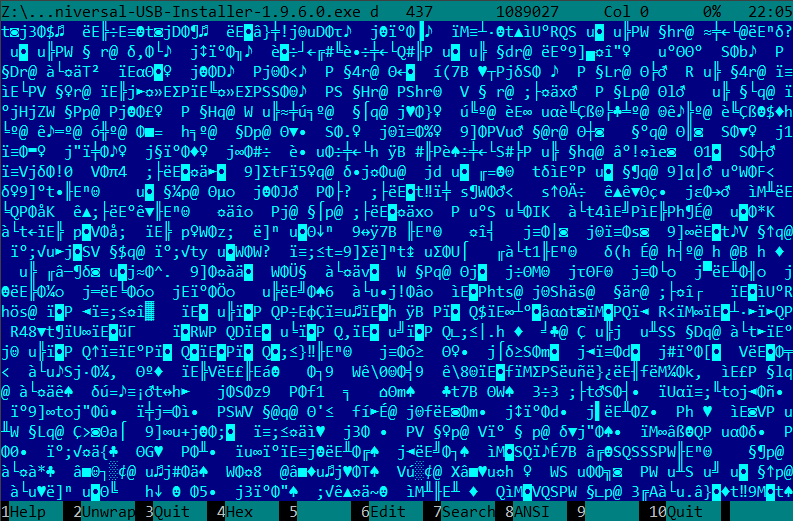
\includegraphics[scale=\NormalScale]{digging_into_code/binary/x86_32.png}
\caption{FAR: \EN{Executable 32-bit x86 code}\RU{Исполняемый 32-битных x86 код}}
\end{figure}

% TODO: Read more about x86 statistics: \ref{}. % FIXME blog post about decryption...

\clearpage
\subsection{\EN{BMP graphics files}\RU{Графические BMP-файлы}}

% TODO: bitmap, bit, group of bits...

\EN{BMP files are not compressed, so each byte (or group of bytes) describes each pixel.
I've found this picture somewhere inside my installed Windows 8.1:}
\RU{BMP-файлы не сжаты, так что каждый байт (или группа байт) описывают каждый пиксель.
Я нашел эту картинку где-то внутри заинсталлированной Windows 8.1:}

\begin{figure}[H]
\centering

\includegraphics[scale=\NormalScale]{digging_into_code/binary/bmp.png}
\caption{\EN{Example picture}\RU{Пример картинки}}
\end{figure}

\EN{You see that this picture has some pixels which probably cannot be compressed very good (around center), 
but there are long one-color lines at top and bottom.
Indeed, lines like these also looks as lines during viewing the file:}
\RU{Вы видите что эта картинка имеет пиксели, которые вероятно не могут быть хорошо сжаты (в районе центра),
но здесь есть длинные одноцветные линии вверху и внизу.
Действительно, линии вроде этих выглядят как линии при просмотре этого файла:}

\begin{figure}[H]
\centering
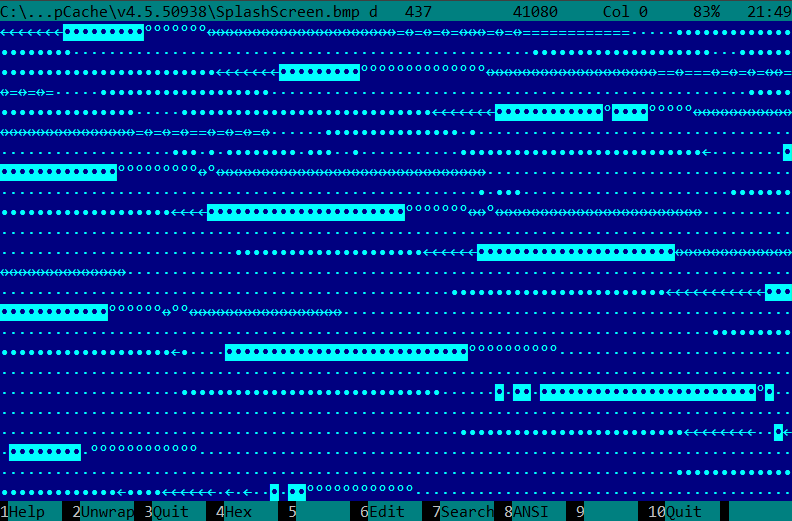
\includegraphics[scale=\NormalScale]{digging_into_code/binary/bmp_FAR.png}
\caption{\RU{Фрагмент BMP-файла}\EN{BMP file fragment}}
\end{figure}

